\section{Introduction}\label{sec:introduction}

For a finite graph \(G\), write \(\alpha(G)\), \(\chi(G)\), and \(h(G)\)
for its independence number, chromatic number, and Hadwiger number.
Thus \(h(G)\) is the largest \(t\) for which \(G\) contains a \(K_t\)
minor.

Hadwiger's conjecture, formulated in 1943~\citep{hadwiger1943},
asserts that \(h(G)\ge\chi(G)\) for every finite nonempty simple
graph \(G\). We disprove it using graphs of independence number
at most two.

Two disjoint edges are \emph{touching} if an edge joins their
endpoint sets. A \emph{connected matching} is a matching whose edges
are pairwise touching; write \(\cm(G)\) for its maximum size. The word
connected in this definition requires adjacency of every pair of
matching edges.

Our main result is the following.
\begin{theorem}\label{thm:main}
There are arbitrarily large integers \(m\) for which an \(m\)-vertex
finite simple graph \(G\) satisfies
\[
             \alpha(G)\le2
             \qquad\text{and}\qquad
             \cm(G)<\frac{m}{100}.
\]
\end{theorem}

A complete minor with many singleton or two-vertex branch sets gives
a large connected matching. The precise counting inequality, proved in
\Cref{prop:matching-minor}, is
\[
                    h(G)\le\frac{|V(G)|+4\cm(G)+2}{3}.
\]
Every color class has size at most \(\alpha(G)\), so
\(\chi(G)\ge |V(G)|/\alpha(G)\). The same lower bound holds
for fractional coloring, giving a second consequence of the construction.
For a finite nonempty simple graph \(G\), let \(\mathcal I(G)\) be
the family of its independent vertex sets. A fractional coloring
assigns a nonnegative real weight \(w_I\) to every \(I\in\mathcal I(G)\)
such that \(\sum_{I\ni v}w_I\ge1\) for every vertex \(v\).
The ordinary fractional chromatic number \(\chi_f(G)\) is the minimum
of \(\sum_Iw_I\) over these assignments.
An ordinary coloring gives a fractional coloring with unit weights
on its color classes, so \(\chi_f(G)\le\chi(G)\).

\begin{corollary}\label{cor:hadwiger}\label{cor:fractional-hadwiger}
There are finite nonempty simple graphs \(G\) of arbitrarily large
order \(m\) for which
\[
 h(G)<\frac{26m}{75}+\frac23
 <\frac m2\le\chi_f(G)\le\chi(G).
\]
Thus Hadwiger's conjecture and its fractional-coloring weakening
\(\chi_f(G)\le h(G)\) are false.
\end{corollary}
\begin{proof}
Summing the vertex constraints of any fractional coloring gives
\[
 |V(G)|\le\sum_{I\in\mathcal I(G)}|I|w_I
       \le\alpha(G)\sum_{I\in\mathcal I(G)}w_I.
\]
Hence \(\chi_f(G)\ge |V(G)|/\alpha(G)\). Apply
\Cref{thm:main} and the minor bound above, noting that
\(26m/75+2/3<m/2\) for \(m\ge5\).
\end{proof}

\citet[p.~148]{reedseymour1998} discussed the weakening that, for every
positive integer \(p\), a graph with no \(K_{p+1}\) minor should have
a fractional \(p\)-coloring,
and proved the corresponding \(2p\)-bound in their result (1.3).
Their convention uses nonnegative rational weights, coverage exactly
one at each vertex, and total weight at most \(p\), so every such
coloring is admissible above. Taking \(p=h(G)\) in the corollary
therefore disproves this prediction as well. The relaxation is on the
coloring side; \(h(G)\) remains the ordinary clique-minor number.

\subsection{Historical context}

Hadwiger's conjecture places planar coloring in a broader minor-theoretic
setting. The \(K_4\)-minor-free case was proved independently by
Hadwiger~\citep{hadwiger1943} and Dirac~\citep{Dirac1952}.
Wagner's structure theorem~\citep{Wagner1937} makes the
four-colorability of graphs without a \(K_5\) minor equivalent to the
Four-Color Theorem, proved by Appel and Haken, with Koch contributing
to the reducibility part~\citep{AppelHaken1977,AppelHakenKoch1977}.
Robertson, Seymour, and Thomas~\citep{RobertsonSeymourThomas1993}
proved that every graph without a \(K_6\) minor is five-colorable,
by reducing the obstruction to a graph that becomes planar after
one vertex is removed. These results explain the conjecture's link
between coloring and the structure of minor-closed classes.

For general \(t\), the density bounds of
Kostochka~\citep{Kostochka1984} and Thomason~\citep{Thomason1984}
give \(O(t\sqrt{\log t})\)-colorability for graphs with no \(K_t\)
minor. Norin, Postle, and Song~\citep[Theorem~1.4]{NorinPostleSong2023}
broke this degeneracy barrier, obtaining
\(O(t(\log t)^\beta)\) colors for every fixed \(\beta>1/4\).
Delcourt and Postle~\citep[Theorem~1.5]{DelcourtPostle2025} reduced the
bound to \(O(t\log\log t)\). A recent preprint of Liu and
Luo~\citep[Theorem~1.1]{LiuLuo2026} further gives
\(O(t\log\log\log t)\)-colorability.

The restriction of Hadwiger's conjecture to graphs of independence
number at most two has an equivalent formulation: every such
graph on \(m\) vertices should have a
\(K_{\lceil m/2\rceil}\) minor. Plummer, Stiebitz, and
Toft~\citep[Theorem~3.1]{pst2003} proved equivalence between the
restricted conjecture and this universally quantified minor assertion.
This identifies the case
\(\alpha(G)\le2\) as a setting in which chromatic number can be replaced by an
explicit fraction of the order.

Duchet and Meyniel~\citep{duchet1982} proved the general lower bound
\(h(G)\ge |V(G)|/(2\alpha(G)-1)\), giving \(h(G)\ge m/3\)
when \(\alpha(G)=2\). Blasiak~\citep{Blasiak2007} obtained complete-minor models of order
\(\Omega(m^{4/5})\) using only singleton and edge branch sets.
Fox~\citep[Theorem~2]{fox2010} strengthened the \(m/3\) bound to
\[
             h(G)\ge \frac m3+c\,m^{4/5}(\log m)^{1/5}
\]
for an absolute constant \(c>0\). His Theorem~3 also yields a
connected matching of size \(\Omega(m^{4/5}(\log m)^{1/5})\), since
its alternative clique of the same order can be paired. These bounds
describe the quantitative background
to the fixed linear upper bounds in \Cref{thm:main,cor:hadwiger}.

F\"uredi, Gy\'arf\'as, and Simonyi~\citep{fgs2005}
proposed the sharp connected-matching conjecture: a graph with
independence number two and order \(4t-1\) has a connected matching
of size \(t\). They verified the assertion through \(t=17\),
and Chen and Deng~\citep{ChenDeng2025} extended this
range to \(t=22\). Cambie~\citep[Theorem~1.5]{cambie2021} proved that
Hadwiger's conjecture implies this statement. The graphs in
\Cref{thm:main} also disprove the sharp connected-matching conjecture:
delete at most three vertices to obtain order \(4t-1\); the
connected-matching number does not increase and remains below \(t\)
for sufficiently large orders. The remaining graph has independence
number exactly two, since a complete graph of order \(4t-1\) has a
connected matching of size \(2t-1\).

Substantial positive results also come from additional clique structure.
Chudnovsky and Seymour~\citep[Theorem~1.3]{ChudnovskySeymour2012}
proved that an \(m\)-vertex graph with independence number at most two
has a \(K_{\lceil m/2\rceil}\) minor whenever its clique number is
at least \(m/4\) for even \(m\), or at least \((m+3)/4\) for odd
\(m\). Their method packs induced three-vertex paths. Norin and
Seymour~\citep[Theorem~1.2]{NorinSeymour2026} subsequently combined this
structure with random pairing to obtain minors of order \(\chi(G)\)
and edge density at least \(\gamma-o(1)\), where
\(\gamma=0.986882\ldots\) is a fixed constant.
These results highlight the requirement in a complete-minor model:
every pair of branch sets must be joined, whereas high density permits
missing adjacencies.

A weaker conjecture asks only for some absolute \(c_0>0\) such that
\(\cm(G)\ge c_0|V(G)|\) for all sufficiently large graphs with
\(\alpha(G)\le2\)~\citep{fgs2005}.
Yip~\citep[Theorem~7]{yip2025} proved a dense variant: a matching of
linear size can have the proportion of its non-touching edge pairs
made arbitrarily small, with the linear coefficient depending on the
prescribed proportion. That statement allows such pairs to remain.
The fixed coefficient in \Cref{thm:main} leaves the weaker conjecture
for smaller positive coefficients unresolved; it does not assert
\(\cm(G)=o(|V(G)|)\).

A related parity-constrained problem has a different recent resolution.
An odd \(K_t\) minor consists of \(t\) disjoint trees, each properly
two-colored, with a same-color edge joining every pair of trees.
K\"uhn, Sauermann, Steiner, and Wigderson~\citep{KuhnSauermannSteinerWigderson2025}
disproved the odd Hadwiger conjecture using graphs of independence
number at most two. The construction in this paper bounds the order
of ordinary complete minors.

The separate companion manuscript~\citep[Theorem~1.1]{OpenAIColinDeVerdiereCounterexample2026}
constructs graphs with \(\chi(G)>\mu(G)+1\), where \(\mu\) is the
ordinary Colin de Verdi\`ere invariant. Since \(h(G)\le\mu(G)+1\),
its result also gives counterexamples to Hadwiger's inequality.
The argument here proves the connected-matching bound directly and
does not use that invariant.


\subsection{The construction and its proof}

We build \(G\) by sampling from a finite probability space and
declaring some pairs to be \emph{holes}, or missing edges. The hole
relation has no loops or triangles. Its complement on the sampled
positions therefore has independence number at most two, even when
sampled elements repeat. An ordered pair with no internal hole is
called a \emph{unit}; it represents a possible matching edge.
Two units conflict when all four cross pairs are holes, as in
\Cref{fig:four-holes}. Such edges cannot belong to one connected
matching.

The main distribution theorem forces conflicts between independent
units drawn from any law with specified marginal and joint density
bounds. It permits arbitrary dependence between the endpoints of a
unit, as is necessary when the units come from a matching. An
entropy-minimizing container argument transfers this statement to the
finite sample: while a family of units supports such a law,
supersaturation supplies a conflict neighborhood to delete; when no
such law remains, a capacitated cut covers the residual family by a
small set of endpoint types and a small set of pairs.

\begin{figure}[htbp]
\centering
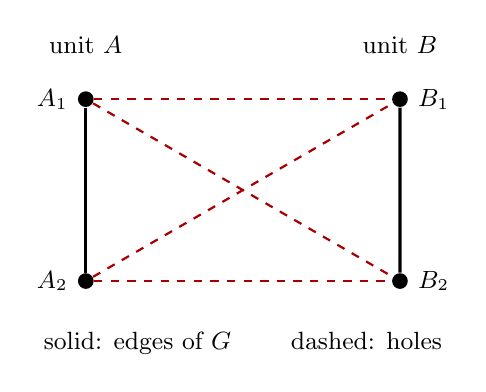
\begin{tikzpicture}[scale=1.05,every node/.style={font=\small}]
\node[circle,fill=black,inner sep=2pt,label=left:$A_1$] (a1) at (0,1.1) {};
\node[circle,fill=black,inner sep=2pt,label=left:$A_2$] (a2) at (0,-1.1) {};
\node[circle,fill=black,inner sep=2pt,label=right:$B_1$] (b1) at (3.8,1.1) {};
\node[circle,fill=black,inner sep=2pt,label=right:$B_2$] (b2) at (3.8,-1.1) {};
\draw[very thick] (a1)--(a2);
\draw[very thick] (b1)--(b2);
\draw[dashed,thick,red!65!black] (a1)--(b1);
\draw[dashed,thick,red!65!black] (a1)--(b2);
\draw[dashed,thick,red!65!black] (a2)--(b1);
\draw[dashed,thick,red!65!black] (a2)--(b2);
\node at (0,1.75) {unit \(A\)};
\node at (3.8,1.75) {unit \(B\)};
\node[align=center] at (1.9,-1.85)
{solid: edges of \(G\) \qquad dashed: holes};
\end{tikzpicture}
\caption{All four cross holes make the two solid matching edges
non-touching. The distribution theorem forces this conflict in every
unit law satisfying its marginal and joint density bounds.}
\label{fig:four-holes}
\end{figure}

To define holes, each sampled configuration carries injective linear
maps into common binary vector spaces. The coefficient spaces record
monomial evaluations \(v\) at Boolean points; their point moments
are the rank-one matrices \(vv\trans\). The frame maps induce an
embedding \(U_o\) of a space built from these moments, together with
a linear functional \(u_o\) on the ambient tensor space. Auxiliary
frame columns will be used to impose the cross-contraction equations.
A hole is certified by a shared tensor and two prescribed identities for the cross
contractions. The identities come from a symmetric bilinear form;
summing them around a hypothetical triangle cancels every bilinear
term and leaves \(0=1\). \Cref{sec:geometry} proves this parity
mechanism before constructing the particular moments and frames.

Forcing four holes is the harder task. The construction has one
unbounded parameter \(n\), and the ambient vector dimension is
\(N=M_0n\), with \(M_0\) fixed before the limit. The three main
steps are as follows.

\begin{enumerate}
\item
\emph{Finite certificates for four holes
(\Cref{sec:moments,sec:realization,sec:collision}).}
The candidate witnesses are short sums of point moments. A point's
\emph{key} is the tuple of its images under the relevant frame maps;
equal keys on the two sides give a shared tensor. We retain specified
images of a bounded number of coefficient directions, called
\emph{pins}. A fixed Boolean selector labels the points;
interpolation and a bounded set of excluded labels make the key
directions independent modulo these pins. A separate low-rank
moment decomposition identifies the obstructions to solving the
cross-contraction equations. Once the corresponding scalar conditions
hold, the remaining equations cost only \(O(n)\) bits. The collision
criterion in \Cref{prop:collision} reduces four holes to overlap of
the accepted key distributions. The witness sums use paired lists of
points, and a \emph{scalar recipe} prescribes their scalar conditions.
Sampling the point parameters with the configuration fixed will be
called a \emph{query}; its full key is the list of the point keys.

\item
\emph{Preparation of the unit law
(\Cref{sec:phases,sec:preparation}).}
Conditioning on exact pin images decomposes the law into parts called
\emph{leaves}, with control of every further independent image
prescription. A \emph{small table} records the cross pairings of the
projected pin directions and the auxiliary frame directions. The
scalar conditions must be compatible with this table. Phase estimates
produce compatible tables on a positive mass of independent unit
pairs, or on a smaller mass at least a fixed multiple of \(N^{-4}\)
determined by their leaves.

\item
\emph{Forcing overlap
(\Cref{sec:histograms,sec:product-tests,sec:common-limit,sec:status-span,sec:rare-overlap}).}
Each leaf's accepted key distributions have finite \(L^1\)
approximating families. Estimates for the mixed law also control
tests of single keys and the scalar values recorded with them.
A product comparison connects these single-position estimates to
tests of the full key tuple. If overlap vanished in the positive-mass
case, a common limit would rule out every scalar recipe whose matched
positions have positive overlap; finite-dimensional duality produces
precisely such a recipe. The inverse-polynomial compatibility mass
may disappear in this limit, so it is handled separately: a uniform large-set
estimate is applied to a finite family chosen on one leaf before
the independent opposite leaf is sampled.
\end{enumerate}

The Boolean moment argument uses commuting multiplication operators,
as in the flat-extension approach to moment problems
\citep{laurentmourrain2009}. The distribution-to-graph argument
combines information projection~\citep{csiszar1975}, independent-set
fingerprints~\citep{kleitmanwinston1982,samotij2015}, and a capacitated
cut~\citep{fordfulkerson1956}. The overlap estimates use entropy
\citep{cover2006} and the energy-increment method of weak regularity
\citep{frieze1999}; the additional constraints from the frame pairings
are retained explicitly in their proofs.

\subsection{Organization and conventions}

\Cref{sec:geometry,sec:distributions} define the frames and holes and
reduce the graph problem to uniform supersaturation.
\Cref{sec:frame-laws} establishes the frame-image estimates and the
decomposition into pinned leaves.
\Cref{sec:moments,sec:realization,sec:collision} prove the algebraic
realization and collision criteria.
\Cref{sec:phases,sec:preparation} prepare the unit law and its small
tables. The analytic comparison tools are established in
\Cref{sec:histograms,sec:product-tests}.
\Cref{sec:common-limit,sec:status-span} prove overlap on the branches
with positive limiting compatibility mass, and
\Cref{sec:rare-overlap} handles the remaining branch and completes the
proof. \Cref{sec:parameters} collects the order of choices and the
quantitative margins.

All vector spaces, matrices, ranks, and algebraic forms are over
\(\F\). Probabilities, densities, norms, and entropies are real.
Logarithms in bit counts have base two; changing the base for entropy
only changes fixed constants.
Constants described as bounded may be very large but are independent
of \(n\). An \(O(n)\) scalar record has its coefficient fixed before
\(M_0\) is chosen. Later fixed test accuracies and partition sizes may
change how large \(n\) must be; they do not change the construction.

The two endpoints in one unit may be dependent. Separate units, and
their leaves before additional pairing conditions, are sampled
independently. Query subdensities retain the mass lost to all
acceptance tests.
